\begin{frame}{Metode iterasi titik-tetap (\textit{fixed-point} iteration)}
\fontsize{10}{11}\selectfont

Metode iterasi titik-tetap adalah salah satu dari metode terbuka untuk menghitung
akar dari persamaan nonlinear.
Langkah pertama dari metode ini adalah menuliskan kembali persamaan
$f(x) = 0$ menjadi:
\begin{equation}
x = g(x)  
\label{eq:x_gx}
\end{equation}
Jika $x$ merupakan akar dari $f(x)$ maka Persamaan \eqref{eq:x_gx}
juga akan terpenuhi. Artinya jika kita dapat menemukan $x$ sedemikan rupa sehingga
$x = g(x)$, maka kita telah menemukan akar dari $f(x)$.
Dalam bentuk iterasi, metode ini dapat dituliskan sebagai:
$$
x_{i+1} = g(x_{i})
$$
di mana $i$ adalah indeks iterasi. Terdapat beberapa kondisi yang dapat
digunakan untuk menentukan konvergensi. Salah satunya adalah dengan
menggunakan estimasi galat
$$
\epsilon_{a} = \left| \frac{x_{i+1} - x_{i}}{x_{i+1}} \right|
$$
Iterasi dihentikan jika $\epsilon_{a}$ lebih kecil dari suatu nilai
tertentu.
\end{frame}


\begin{frame}
\fontsize{9}{10}\selectfont

\begin{block}{Contoh metode iterasi titik-tetap}
Gunakan metode iterasi titik-tetap untuk mencari akar dari
$f(x) = e^{-x} - x$
\end{block}
Fungsi $f(x)$ diubah dulu mejadi $x = g(x)$ di mana $g(x) = e^{-x}$.
Iterasi titik-tetap memberikan skema iterasi:
$$
x_{i+1} = e^{-x_{i}}
$$
Dengan nilai awal $x_0 = 0$ diperoleh iterasi seperti pada tabel berikut.

{\centering
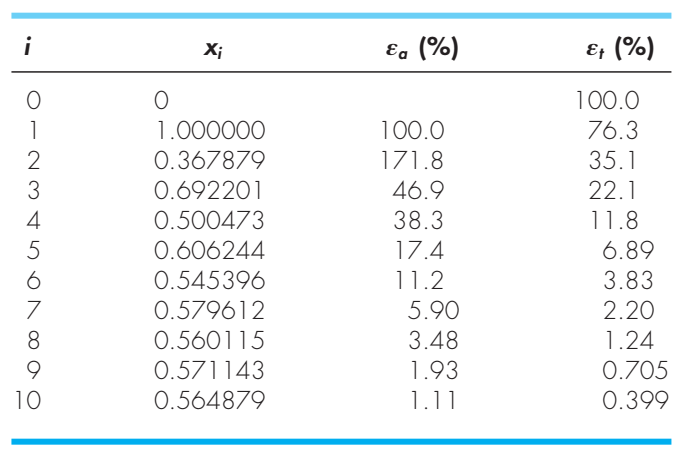
\includegraphics[height=0.5\textheight]{../chapra_7th/Chapra_Table_Example_6_1.png}
\par}

\end{frame}


\begin{frame}{Interpretasi grafis}
\fontsize{10}{11}\selectfont

\begin{columns}

  \begin{column}{0.5\textwidth}
  {\centering
  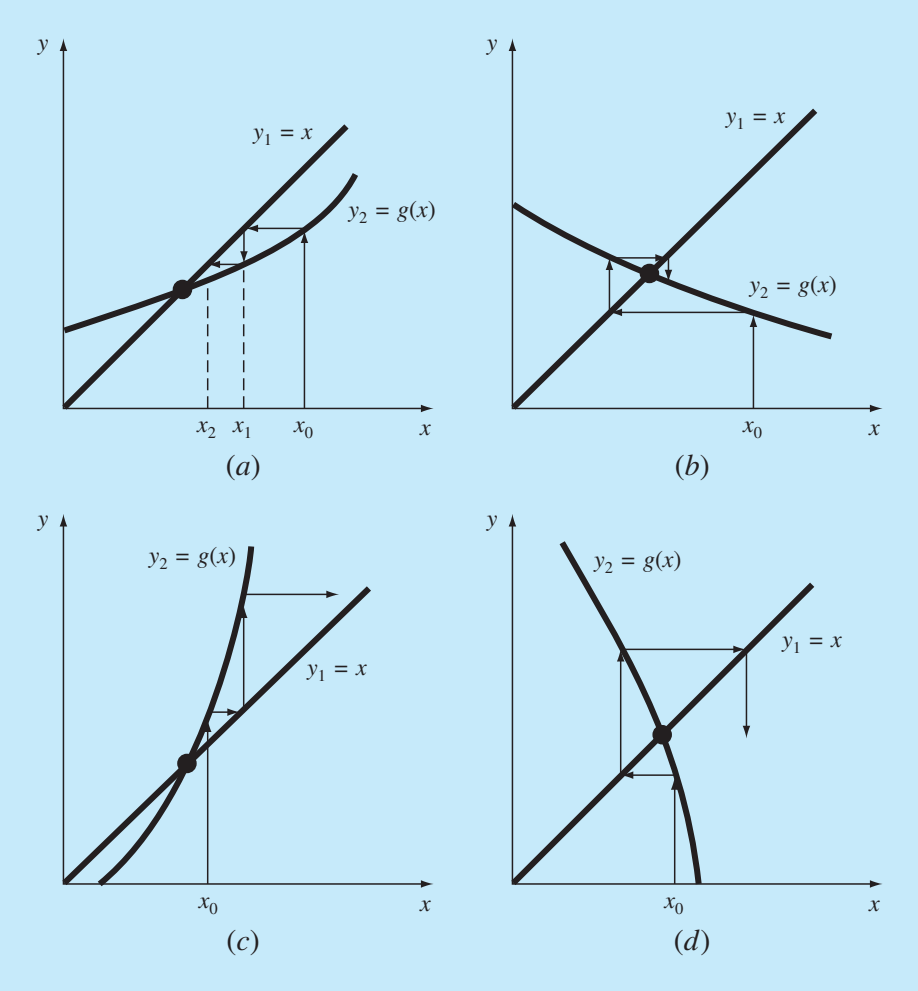
\includegraphics[height=0.8\textheight]{../chapra_7th/Chapra_Fig_6_3.png}
  \par}
  \end{column}

  \begin{column}{0.5\textwidth}
  Secara grafis, metode iterasi titik-tetap bertujuan untuk
  menemukan perpotongan antara kurva $y_1 = x$ dengan
  kurva $y_2 = g(x)$.

  Metode iterasi titik-tetap tidak selalu konvergen.

  Dari gambar, terlihat bahwa iterasi titik-tetap akan konvergen jika
  $|g'(x) < 1|$: magnitudo dari kemiringan $g(x)$ lebih kecil daripada
  kemiringan garis $y_1 = x$ pada daerah di mana metode ini diaplikasikan.
  \end{column}
\end{columns}

\end{frame}


\begin{frame}
\fontsize{9}{10}\selectfont

Skema iterasi:
$$
x_{i+1} = g(x_{i})
$$
Misalkan solusi dari iterasi titik-tetap ini adalah $x_r$, sehingga berlaku:
$$
x_{r} = g(x_r)
$$
Dengan mengurangi kedua persamaan tersebut diperoleh:
\begin{equation}
x_r - x_{i+1} = g(x_r) - g(x_i)
\label{eq:B6_1_1}
\end{equation}

Menggunakan teorema nilai rata-rata turunan: jika suatu fungsi $g(x)$
dan turunan pertamanya kontinu pada suatu interval $a \leq x \leq b$,
maka terdapat setidaknya satu nilai $x = \xi$ dalam interval tersebut
sedemikian rupa sehingga:
\begin{equation}
g'(\xi) = \frac{g(b) - g(a)}{b - a}
\label{eq:B6_1_2}  
\end{equation}
Ruas kanan dari persamaan ini adalah kemiringan dari garis yang menghubungkan antara
$g(a)$ dan $g(b)$. Dengan kata lain, teorema rata-rata turunan menyatakan bahwa
setidaknya ada satu titik di antara $a$ dan $b$ yang memiliki kemiringan,
$g'(\xi)$, yang sejajar dengan garis yang menghubugkan antara $g(a)$ dan
$g(b)$.
\end{frame}


\begin{frame}
\fontsize{9}{10}\selectfont

Jika $a = x_{i}$ dan $b = x_r$, maka ruas kanan dari
Persamaan \eqref{eq:B6_1_1} dapat dituliskan sebagai:
\begin{equation*}
g(x_r) - g(x_i) = (x_r - x_i) g'(\xi)
\end{equation*}
sehingga Persamaan \eqref{eq:B6_1_1} dapat dituliskan juga menjadi:
\begin{equation}
x_r - x_{i+1} = (x_r - x_i) g'(\xi)
\end{equation}
Dengan definisi galat sebenarnya untuk iterasi ke-$i$ sebagai:
$$
E_{t,i} = x_r - x_i
$$
maka:
$$
E_{t,i+1} = g'(\xi) E_{t,i}
$$
Dari persamaan ini dapat dilihat bahwa galat akan semakin berkurang pada
setiap iterasi jika $|g'(x)| < 1$. Sebaliknya, jika $|g'(x)| > 1$
galat akan semakin membesar.

Selain itu, jika turunan bernilai positif, maka galat akan positif solusi iteratif
akan monotonik. Jika turunan bernilai negatif, maka galat akan berosilasi.

Analisis ini juga menunjukkan bahwa galat pada metode iterasi titik-tetap akan
sebanding dengan galat dari langkah sebelumnya. Oleh karena ini iterasi titik-tetap
dikatakan memiliki sifat konvergensi linear (\textit{linearly convergent}).
\end{frame}


\begin{frame}{Metode Newton-Raphson}
\fontsize{9}{10}\selectfont

\begin{columns}

  \begin{column}{0.5\textwidth}
  Metode Newton-Raphson mungkin adalah metode yang paling terkenal
  di antara metode pencarian akar linear.

  Pada metode ini jika kita mulai dari tebakan akar $x_i$, kita dapat menarik garis
  singgung (\textit{tangent line})
  dari titik $(x_i, f(x_i))$. Titik perpotongan antara garis singgung ini
  dengan sumbu-$x$ merupakan tebakan selanjutnya untuk akar.
  
  Dari gambar dapat dicari garis singgung pada $x_i$:
  $$
  f'(x_{i}) = \frac{f(x_i) - 0}{x_i - x_{i+1}}
  $$
  diperoleh:
  \begin{equation}
  \myhighlight{
  x_{i+1} = x_{i} - \frac{f(x_{i})}{f'(x_{i})}
  }\label{eq:Chapra_6_6}
  \end{equation}
  Metode ini dapat digunakan jika $f'(x_{i}) \neq 0$.
  \end{column}

  \begin{column}{0.5\textwidth}
  {\centering
  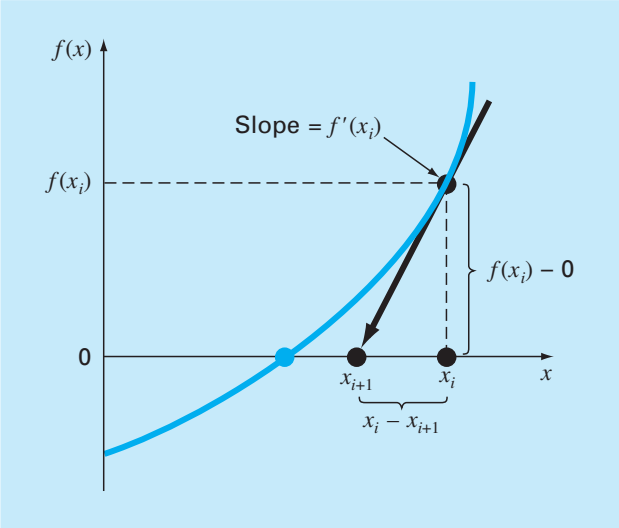
\includegraphics[height=0.8\textheight]{../chapra_7th/Chapra_Fig_6_5.png}
  \par}
  \end{column}

\end{columns}

\end{frame}


\begin{frame}
\fontsize{10}{11}\selectfont

\begin{block}{Contoh}
Gunakan metode Newton-Raphson untuk mengestimasi akar dari $f(x) = e^{-x} - x$ dengan
menggunakan tebakan akar awal $x_{0} = 0$.
\end{block}

Kita perlu mencari $f'(x)$ terlebih dahulu:
$$
f'(x) = -e^{-x} - 1
$$
Dengan menggunakan skema iterasi pada Persamaan \eqref{eq:Chapra_6_6} diperoleh
hasil pada tabel berikut.

{\centering
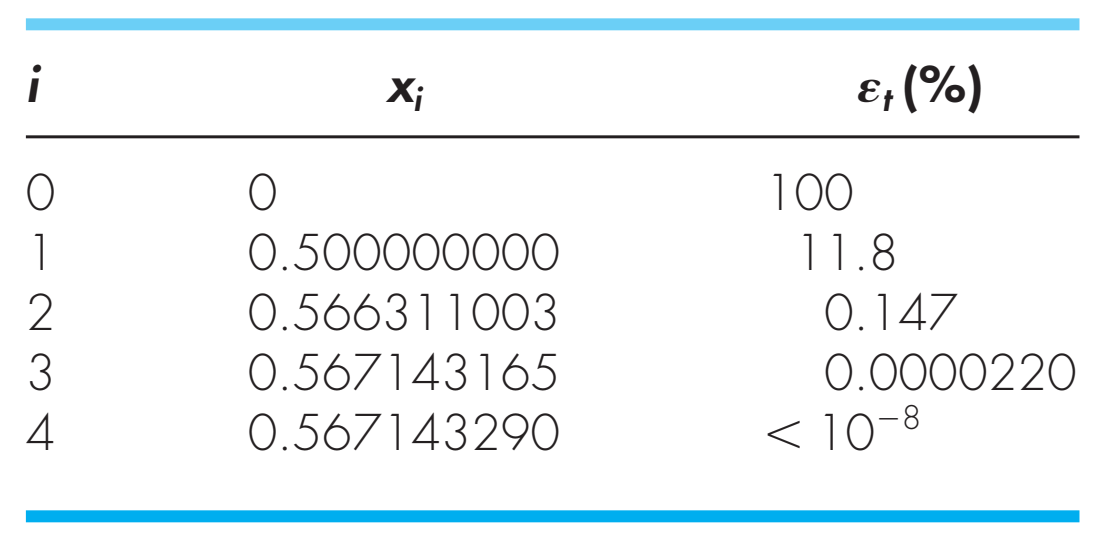
\includegraphics[height=0.4\textheight]{../chapra_7th/Chapra_Table_Example_6_3.png}
\par}

\end{frame}


\begin{frame}
\fontsize{9}{10}\selectfont

\begin{columns}
  \begin{column}{0.5\textwidth}
  \begin{block}{Contoh}
  Tentukan akar positif dari $f(x) = x^{10} - 1$ dengan menggunakan metode Newton-Raphson
  dan tebakan awal $x_0 = 0.5$.
  \end{block}
  Biasanya metode Newton-Raphson konvergen ke akar dengan cepat (konvergensi kuadratik).
  Namun pada kasus tertentu, seperti pada contoh ini,
  metode Newton-Raphson dapat kesulitan untuk konvergen.
  
  Skema iterasi Newton-Raphson pada kasus ini dapat dituliskan sebagai berikut:
  $$
  x_{i+1} = x_{i} - \frac{x_{i}^{10} - 1}{10x_{i}^{9}}
  $$
  Diperoleh hasil pada tabel berikut.
  \end{column}

  \begin{column}{0.5\textwidth}
  
  {\centering
  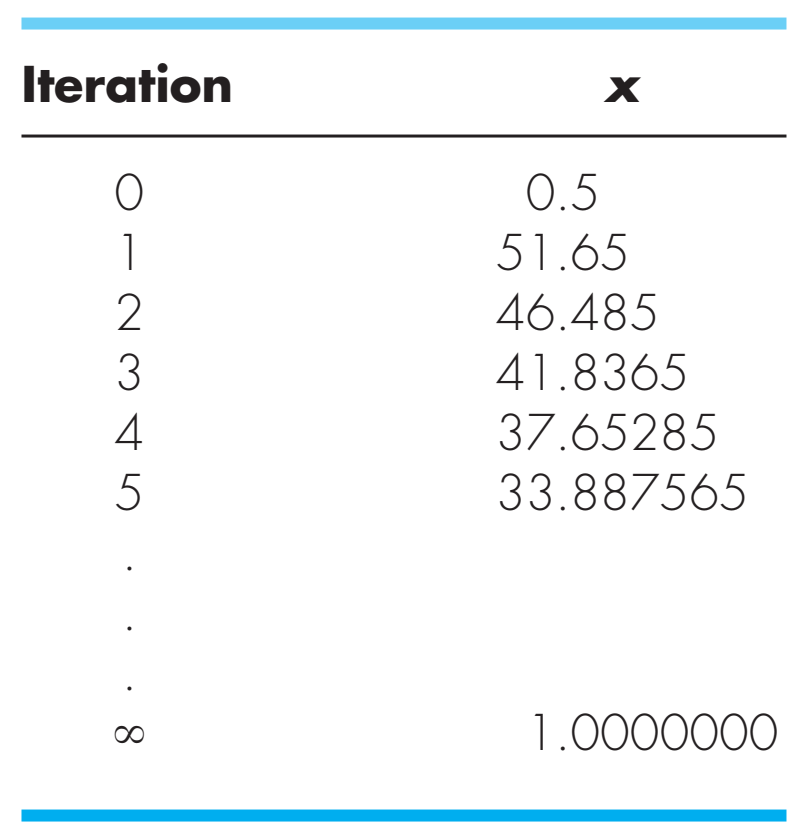
\includegraphics[height=0.5\textheight]{../chapra_7th/Chapra_Table_Example_6_5.png}
  \par}

  Seperti terlihat pada tabel, metode Newton-Raphson konvergen sangat lambat ke
  akar.

  Penyebab dari konvergensi yang lambat ini dapat didiagnosa
  dengan cara membuat plot dari fungsi yang bersangkutan.
  Biasanya dapat terjadi osilasi atau nilai tebakan akar yang
  jelek dikombinasikan dengan turunan fungsi yang sangat kecil
  (garis singgung yang hampir sejajar dengan sumbu-$x$)
  dapat membuat metode Newton-Raphson kesulitan untuk konvergen.

  \end{column}

\end{columns}

\end{frame}


\begin{frame}{Metode garis-potong (\textit{secant})}

Metode garis-potong mirip dengan metode Newton-Raphson. Perbedaannya
adalah pada metode garis-potong, turunan fungsi diaproksimasi dengan menggunakan
beda-hingga mundur:
$$
f'(x_{i}) \approx \frac{f(x_{i-1}) - f(x_i)}{x_{i-1} - x_{i}}
$$
sehingga diperoleh skema iterasi:
$$
x_{i+1} = x_{i} - \frac{f(x_{i}) (x_{i-1} - x_{i})}{f(x_{i-1}) - f(x_{i})}
$$
Metode garis potong memerlukan dua titik untuk memulai iterasi. Berbeda dengan
metode tertutup, dua titik ini tidak perlu mengapit akar.

\end{frame}



\begin{frame}{Metode garis-potong modifikasi}

Pada metode ini tidak digunakan dua tebakan awal, namun hanya satu titik saja.
Untuk mengaproksimasi turunan, digunakan gangguan kecil:
$$
f'(x_i) \approx \frac{f(x_i + \delta \, x_{i}) - f(x_i)}{\delta \, x_{i}}
$$
atau:
$$
x_{i+1} = x_{i} - \frac{\delta \, x_{i} f(x_i)}{f(x_{i} + \delta \, x_i) - f(x_i)}
$$
dengan $\delta$ adalah suatu bilangan fraksional yang kecil, misalnya $10^{-5}$.

Alternatif lain adalah dengan mengganti keseluruhan $\delta x_{i}$
dengan suatu konstanta yang kecil.

\end{frame}